\documentclass[a4paper, 12pt]{article}
\usepackage{listings} 
\usepackage{xcolor}
\usepackage{mdframed}
\usepackage{graphicx}
\usepackage{pgfplots}
\usepackage{float}
\usepackage{mathtools}
\usepackage[margin=1.00in]{geometry}
\DeclarePairedDelimiter\ceil{\lceil}{\rceil}
\DeclarePairedDelimiter\floor{\lfloor}{\rfloor}

\definecolor{code-gray}{gray}{0.93}
\begin{document}
\title{ECE 443 - Project \#2}
\author{Collin Heist}
\date{\today}
\maketitle
\pagenumbering{roman}
\tableofcontents
\lstlistoflistings
\newpage
\pagenumbering{arabic}

\section{Design Process}
In the previous project I chose to implement a twenty millisecond debounce period using a very rudimentary hardware-assisted delay function, called from inside a change-notice ISR. This worked very well for the first project because there was no need to worry about task execution while the buttons were debouncing, however I had to change my implementation for this project.

I chose to instead call \textbf{vTaskDelay()} inside the change notice handler task. This allows for other tasks to execute, although there are not any other tasks in this program. However, this is still necessary because while the change notice handler task is \emph{blocked} during the duration of that \textbf{vTaskDelay()}, the idle task is performed (as it is the only other 'task'). The idle task's code is shown below, in \textbf{Listing~\ref{lst:idle-task}}

	\begin{mdframed}[backgroundcolor=code-gray, roundcorner=10pt,
								innerleftmargin=5, innertopmargin=5, innerbottommargin=5]	
	\begin{lstlisting}[language=C, caption=Idle Task, tabsize=2, label={lst:idle-task}]
	void vApplicationIdleHook(void) {
		if (PORTG & BTN1)
			mPORTBSetBits(LEDA);
		else
			mPORTBClearBits(LEDA);
	}
	\end{lstlisting}
	\end{mdframed}
	
This idle task ensures that \textbf{LEDA} is always set to the current status of \textbf{BTN1}, and this remains true while the button is being debounced (something that was not occurring in my previous project).

Because the only task that I needed to manually create was my change notice handler task, my choice of task priority was largely arbitrary. But I did take care to set my task priority to a level below that at which interrupts can interrupt (which is by default 3), to ensure the change notice interrupt always took precedence. I chose a task level of 1, which was the lowest task non-idle task priority available.

In order to save the trouble of manually creating a one millisecond toggle \textbf{LEDB} task, which would have created more overhead for task-switching, as well as necessitated more careful planning on my part for task priorities (as the one millisecond toggle would need to occur not matter what), I instead appended my \textbf{LEDB} toggle code onto the existing \textbf{vApplicationTickHook()} functionality.

The function \textbf{vApplicationTickHook()} is automatically called every \textit{tick} of the kernel, which is by default one millisecond. This means that every time the kernel is about to perform a task-switching operation (or even just check if a task should be switched into), my custom tick hook function was called -- giving me the desired one millisecond toggle of \textbf{LEDB}. That code is shown in \textbf{Listing~\ref{lst:tick-hook}}.

\begin{mdframed}[backgroundcolor=code-gray, roundcorner=10pt,
								innerleftmargin=5, innertopmargin=5, innerbottommargin=5]	
	\begin{lstlisting}[language=C, caption=Tick Hook 'Task', tabsize=2, label={lst:tick-hook}]
	void vApplicationTickHook(void) {
		if (configUSE_TRACE_FACILITY) 
			vTracePrint(trace_1ms_task, "Toggling LEDB");
	
		LATBINV = LEDB;
	
		if (configUSE_TRACE_FACILITY && DEBUG_MODE) {
			if (LATB & LEDC)
				trace_ledb_count++;
	
			if (trace_ledb_count >= 2)
				LATB = LATB;
		}
	}
	\end{lstlisting}
	\end{mdframed}
	
The last few lines are what I used in order to obtain my TraceAlyzer screenshot, but overall adding to this kernel tick function was simple. 

Overall, I did not have any problems with this project. The hardest part of this project was setting up TraceAlyzer, as I had to modify parts of the \textbf{FreeRTOS} configuration file, and had a lot of problems having the necessary files in my project directory.
 
\section{Testing \& Verification}
In order to verify the operation of my code, I used the TraceAlyzer plugin for \textbf{FreeRTOS}. The project outline had me finish a capture once \textbf{LEDB} had been toggled twice while \textbf{LEDD} was lit. That resulted in the event log showed in \textbf{Figure~\ref{fig:pic-tracealyzer-button-press}}.

\begin{figure}[H]
\centering
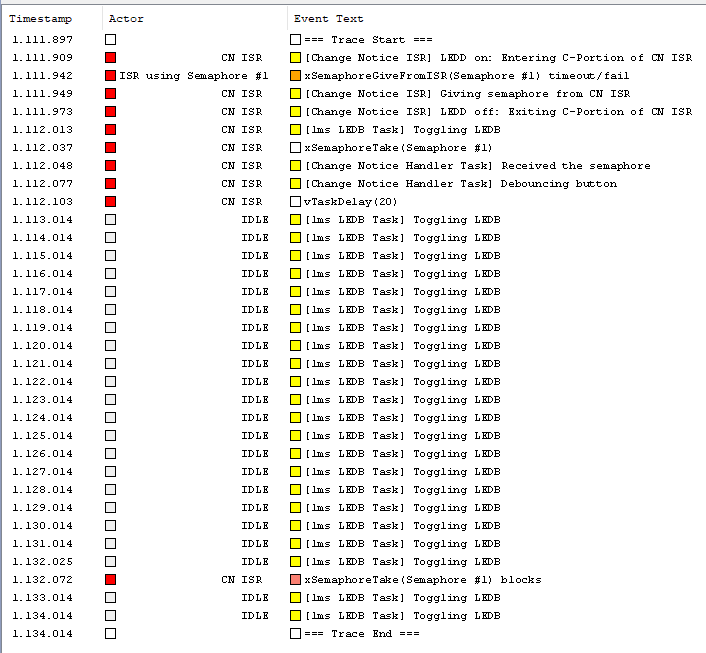
\includegraphics[width=0.9\textwidth]{pic-tracealyzer-button-press.PNG}
\caption{TraceAlyzer event log of two \textbf{LEDB} toggles after a button press}
\label{fig:pic-tracealyzer-button-press}
\end{figure}

As evident in the picture, once the button is pressed, the sequence of events occurred as follows: 

\begin{enumerate}
\item The C-portion of the ISR is executed
\item The timing worked out such that a previous call of \textbf{xSemaphoreTake()} expired -- this is not a determined event
\item Then, the semaphore was given from the change notice ISR
\item The semaphore was received -- unblocking the change notice handler task
\item The 20ms debounce period began, blocking the handler task
\item 20 milliseconds passed
\item The \textbf{vTaskDelay()} unblocks and quickly blocks again -- waiting for the semaphore once again
\end{enumerate}

This behavior is exactly what is desired based on the project specifications. Which is good!

I also took two captures of the LED pins during a button press and release, also for verification. The first capture shows what happens when a button is first pressed. 

\begin{figure}[H]
\centering
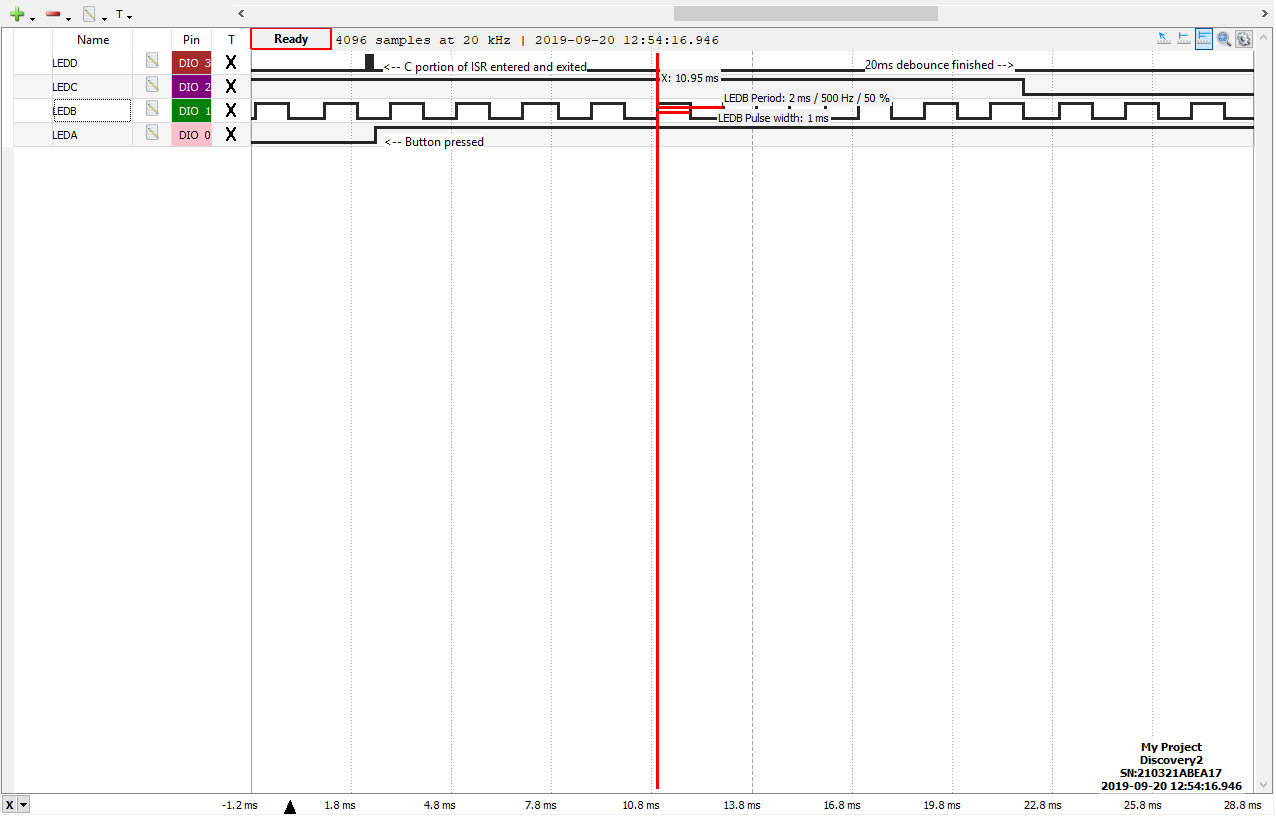
\includegraphics[width=0.9\textwidth]{pic-button-press.png}
\caption{Status of all LED's when a button is \emph{pressed}}
\label{fig:pic-button-press}
\end{figure}

The final figure shows the status of each LED when the button is released.

\begin{figure}[H]
\centering
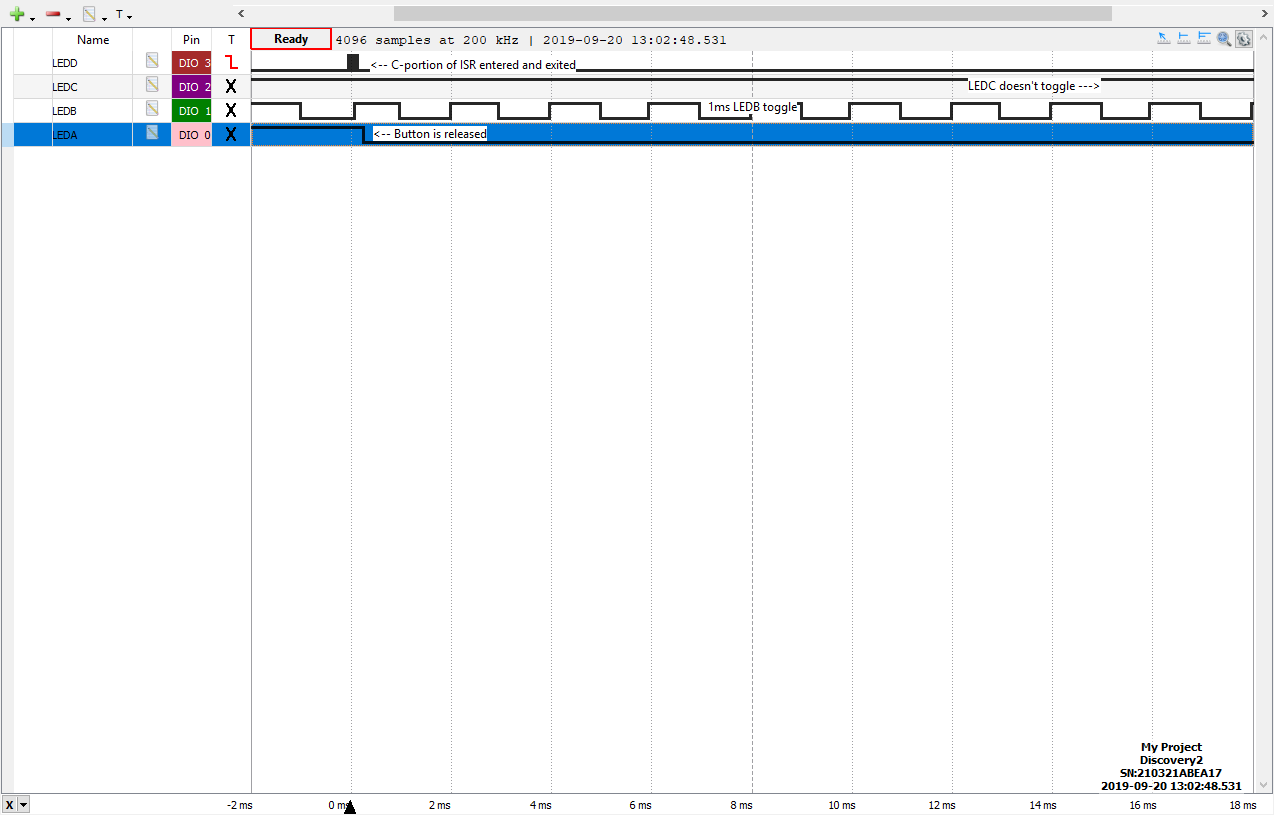
\includegraphics[width=0.9\textwidth]{pic-button-release.png}
\caption{Status of all LED's when a button is \emph{release}}
\label{fig:pic-button-release}
\end{figure}

\end{document}